\documentclass[conference]{IEEEtran}
\IEEEoverridecommandlockouts
% The preceding line is only needed to identify funding in the first footnote. If that is unneeded, please comment it out.
\usepackage{cite}
\usepackage{amsmath,amssymb,amsfonts}
\usepackage{algorithmic}
\usepackage{graphicx}
\usepackage{textcomp}
\usepackage{xcolor}
\def\BibTeX{{\rm B\kern-.05em{\sc i\kern-.025em b}\kern-.08em
    T\kern-.1667em\lower.7ex\hbox{E}\kern-.125emX}}
\begin{document}

\title{Lunar Landing Simulation using Reinforcement Learning in OpenAI (gym)\\
}

\author{\IEEEauthorblockN{Alfredo J. Peña}
\IEEEauthorblockA{\textit{Department of Computer Science} \\
\textit{University of Texas Rio Grande Valley}\\
Edinburg, Texas \\
alfredo.pena01@utrgv.edu}
\and
\IEEEauthorblockN{Amit Das}
\IEEEauthorblockA{\textit{Department of Computer Science} \\
\textit{University of Texas Rio Grande Valley}\\
Edinburg, Texas \\
amit.das01@utrgv.edu}
\and
\IEEEauthorblockN{Md Shahriar Forhad}
\IEEEauthorblockA{\textit{Industrial \& Manufacturing Engineering} \\
\textit{University of Texas Rio Grande Valley}\\
Edinburg, Texas \\
mdshahriar.forhad01@utrgv.edu}
}

\maketitle

\begin{abstract}
Artificial Intelligence (AI) is considered a very important technology that can analyze a situation or environment and propose related decisions to obtain certain results. It also helps find alternatives and modify actions to changes. It has become popular in process control, finding optimum factors, etc, in different sectors. AI is a very important component of modern industries (Industry 4.0). It is being used in different areas utilizing different sensors like gyro, sonar sensor, light sensor, temperature sensor, GPS, etc.
\end{abstract}

\begin{IEEEkeywords}
lander, space, reinforcement learning, OpenAI
\end{IEEEkeywords}

\section{Introduction}
Artificial Intelligence (AI) is a critical technology that analyzes a situation or environment and makes recommendations to achieve specific outcomes. It also aids in the discovery of alternatives and the adaptation of actions in response to changes. It's become popular in a variety of industries for process control, determining optimum parameters, and so on. Artificial intelligence (AI) is a critical component of today's industry (Industry 4.0). It is utilized in a variety of applications and employs several sensors such as a gyroscope, sonar sensor, light sensor, temperature sensor, GPS, and others.

\section{Background}
Machine learning is a very important part of AI, where different algorithms are studied to train/teach machines. Primarily there are four different types of machine learning algorithm. These are as follows:

\subsection{Supervised}
A set of training data with the labeled outcome is provided in Supervised learning. Historical data, research data can be employed for training the model. A well-labeled data set with distinct features can lead to higher accuracy.

\subsection{Semi-Supervised}
A small set of labeled datasets is combined with a large set of unlabeled datasets to train the model in semi-supervised learning. Comparatively, it has less accuracy than supervised learning algorithms. Semi-supervised learning algorithms help learn from the provided labeled dataset and obtain useful information from the unlabelled dataset \cite{b1}.

\subsection{Unsupervised}
The unlabeled dataset is provided, and the model is assumed to classify the dataset by finding out different features there. It is very challenging to achieve higher accuracy and needs to be provided with a substantial amount of data. The main objectives of unsupervised learning are dimensional reduction, feature extraction and clustering \cite{b2}

\subsection{Reinforcement}
An agent or many agents are designed to make decisions on different available actions in accordance with an environment. According to the actions the agents receive rewards or penalties. The agents aim to get maximum reward and thus it learns about proper actions required for different states of the environment. The agents learn without any supervisor. There are four types of reinforcement learning: positive, negative, punishment, and extinction. Reinforcement learning can be a great tool to optimize certain system parameters. For example, a robotic arm can be trained for 3D motion, classifying and placing objects in their respective areas by employing reinforcement learning \cite{b3}.
\par
\cite{b4} proposed a reinforcement learning and expertise knowledge-based hybrid model to control chiller water temperature.
\par
\cite{b5} reviewed the contribution of reinforcement learning in healthcare.
\par
\cite{b6} stated that due to the uncertainty in the patient's response to the medication, the doctors are not justified to completely depend upon clinical judgment. This can be similed with different industrial processes. There is always a lot of randomness (noise) in most of the system. So, actions are required to be updated in accordance to the changing states.

\begin{figure}[htbp]
\centerline{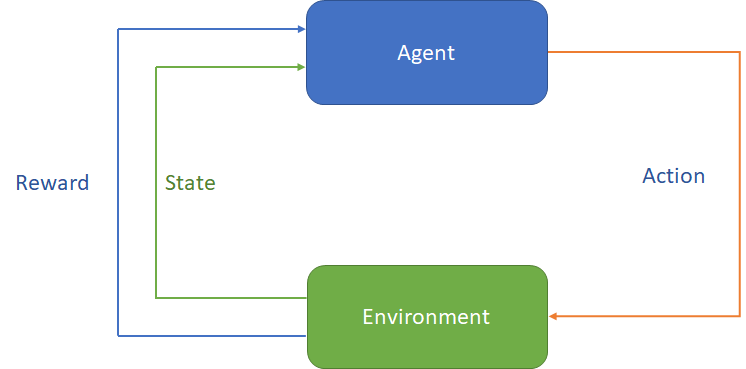
\includegraphics[width=165pt]{images/rl.png}}
\caption{Basic Structure of Reinforcement Learning.}
\label{RL}
\end{figure}

\begin{table*}[t]
\caption{Application of Different Reinforcement Learning Algorithms in Different States\cite{b8}}
\begin{center}
\def\arraystretch{1.5}%
\begin{tabular}{|c|c|c|c|c|c|}
\hline
\textbf{Algorithm}&\textbf{Description}&\textbf{Policy}&\textbf{Action Space}&\textbf{State Space}&\textbf{Operator} \\
\hline
Monte Carlo & Every visit to Monte Carlo & Either & Discrete & Discrete & Sample-Means \\
\hline
Q-learning & State–action–reward–state & Off-Policy & Discrete & Discrete & Q-Value \\
\hline
SARSA & State–action–reward–state–action & On-Policy & Discrete & Discrete & Q-Value \\
\hline
DQN & Deep Q Network & Off-Policy & Discrete & Continuous & Q-Value \\
\hline
DDPG & Deep Deterministic Policy Gradient & Off-Policy & Continuous & Continuous & Q-Value \\
\hline
A3C & Asynchronous Advantage Actor-Critic Algorithm & On-Policy & Continuous & Continuous & Advantage \\
\hline
TRPO & Trust Region Policy Optimization & On-Policy & Continuous & Continuous & Advantage \\
\hline
PPO & Proximal Policy Optimization & On-Policy & Continuous & Continuous & Advantage \\
\hline
TD3 & Twin Delayed Deep Deterministic Policy Gradient & Off-Policy & Continuous & Continuous & Q-Value \\
\hline
\end{tabular}
\label{tab1}
\end{center}
\end{table*}

\section{Deep Learning}
Deep learning is a subfield of ML that is able to extract features without the need for immense data pre-processing or extraction of features and thus has become a competent tool for studying higher-dimensional data \cite{b7}. It can execute complicated assignments with ease. It is a state-of-the-art technology that can imitate the data processing patterns as like as human brain and is playing a significant role in disease screening, diagnosis and prediction \cite{b7}. Besides, deep learning reduces execution time, saves energy consumption in deep neural networks.

\subsection{Advantages of Reinforcement Learning}
Reinforcement learning can reduce the cost of training by employing designed environments even with animation for the user to understand the scenario well. It may seem that the programmed environment might not exactly match the real one, but after training the model in a programmable environment it can learn to adapt to the changes in the real-world experiments. Besides, in some complex processes/ environments, it is very difficult to find out the required solution by developing explicit logic. But, reinforcement learning can find out the optimal solution from out of the box. The decision-making algorithm can be updated as required. Therefore, in an environment where different parameters are altered indefinitely, learning can help adapt to the scenario without explicit supervision.

\subsection{Application of Reinforcement Learning}
Reinforcement learning is widely been used in robotics. In industries, robotics has wide usage in lifting heavy loads, performing monotonous work, completing the complicated task with almost the same accuracy consistently. There are different types of an algorithm for implementing reinforcement learning. The selection of the algorithm is dependent upon different parameters, such as whether action space, state-space is discrete or continuous, etc.

\section{Methodology}

\subsection{The gym Library}
The gym is an open-source library to develop and compare different reinforcement learning algorithms. It is developed with python and R. The gym library has a lot of environments and new environments can be built registered with the library to be implemented for reinforcement learning analysis \cite{b9}.

\subsection{Lunar Lander}
Lunar Lander is a gym environment developed to train reinforcement learning to land a spaceship on land, here on the moon. The gym environment uses a physics formula to calculate the space-ship position and movement. In this environment, the spaceship has three engines: 1: Main engine, 2. Left orientation engine and 3. Right orientation engine. Action space is discrete: 0: Fire no engine, 1: Fire left orientation engine, 2: Fire main engine, 3: Fire right orientation engine. The State Space is continuous with 8 states.

\subsection{DQN}
DQN is a type of reinforcement learning. It combines q-learning and neural networks and helps solve complex environments. It can deal with discrete Action Space and continuous State Space. Therefore, DQN was selected for training the spaceship to land in the Lunar Lander environment. Bellman equation was employed to change the Q-table to be utilized in batch training of the model.

\begin{figure}[hbtp]
\centerline{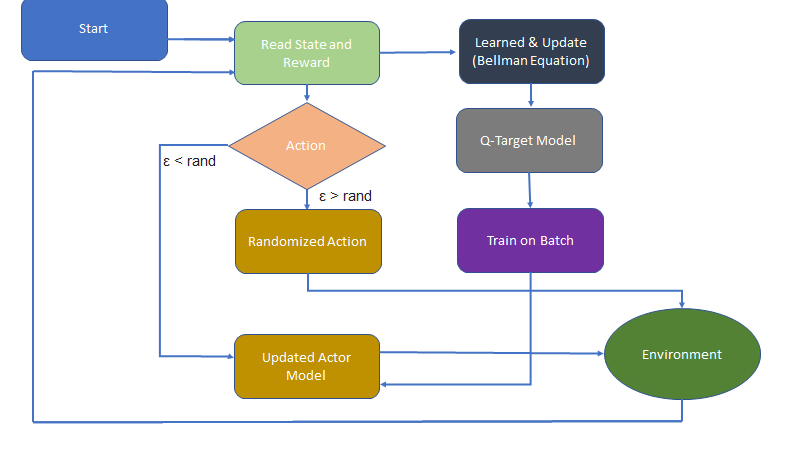
\includegraphics[width=200pt]{images/flow.png}}
\caption{Project Flow Diagram}
\label{FlowDiagram}
\end{figure}

\begin{figure}[hbtp]
\centerline{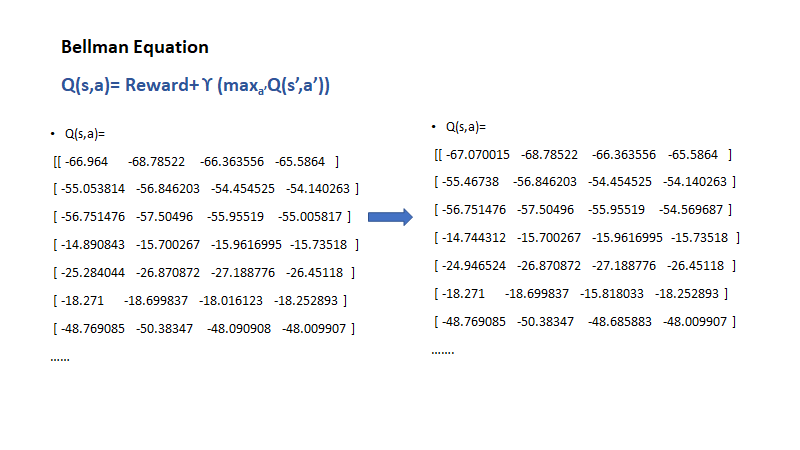
\includegraphics[width=200pt]{images/bellman.png}}
\caption{Bellman Equation and the Change in Q-Table}
\label{Bellman}
\end{figure}

\section{Results and Discussion}
The model was trained well and most of the time it landed safely on the specific region. But the accuracy can be further developed using the Actor-Critic algorithm. Different neural networks were employed during the training. But the result showed that more the dense layer does not necessarily mean more accuracy. At first, the model was trained for 500 episodes with reinforcement learning \cite{b10}. From the episode vs score plot, it seems that after certain episodes the score didn’t increase continuously. Therefore, retrained the model with 200 episodes and found relatively better results. \\ \\ \\ \\

\begin{figure}[hbtp]
\centerline{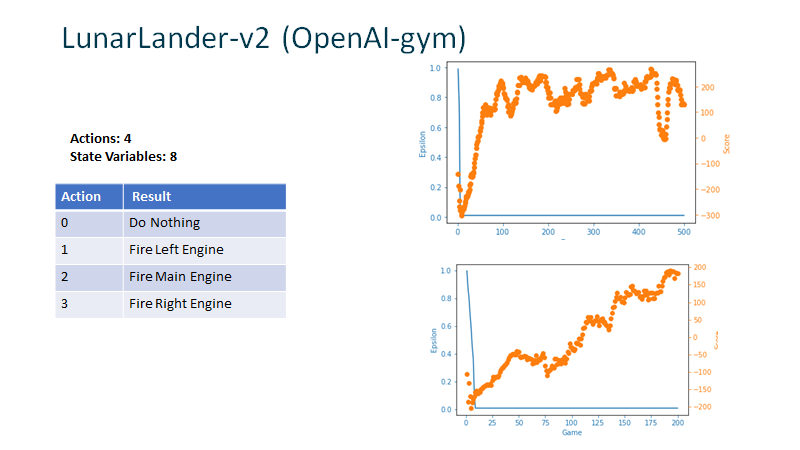
\includegraphics[width=200pt]{images/results1.png}}
\caption{Training the Model with Reinforcement Learning}
\label{TrainResults}
\end{figure}

\begin{figure}[hbtp]
\centerline{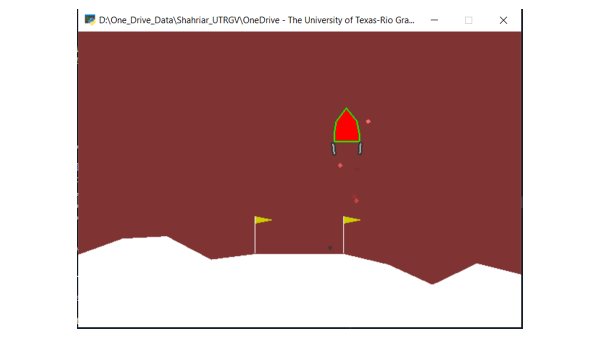
\includegraphics[width=200pt]{images/demo.png}}
\caption{Output of Trained Model}
\label{Demo}
\end{figure}

\begin{thebibliography}{00}
\bibitem{b1} Z. Ge, Z. Song, S. X. Ding, and B. Huang, “Data mining and analytics in the process industry: The role of machine learning,” Ieee Access, vol. 5, pp. 20590–20616, 2017.
\bibitem{b2} R. Nian, J. Liu, and B. Huang, “A review On reinforcement learning: Introduction and applications in industrial process control,” Comput. Chem. Eng., vol. 139, p. 106886, 2020, doi: https://doi.org/10.1016/j.compchemeng.2020.106886. 
\bibitem{b3} M. Matulis and C. Harvey, “A robot arm digital twin utilising reinforcement learning,” Comput. Graph., no. xxxx, pp. 1–9, 2021, doi: 10.1016/j.cag.2021.01.011. 
\bibitem{b4} S. Qiu, Z. Li, D. Fan, R. He, X. Dai, and Z. Li, “Chilled water temperature resetting using model-free reinforcement learning: Engineering application,” Energy Build., vol. 255, p. 111694, 2022, doi: https://doi.org/10.1016/j.enbuild.2021.111694. 
\bibitem{b5} A. Coronato, M. Naeem, G. De Pietro, and G. Paragliola, “Reinforcement learning for intelligent healthcare applications: A survey,” Artif. Intell. Med., vol. 109, p. 101964, 2020, doi: https://doi.org/10.1016/j.artmed.2020.101964. 
\bibitem{b6} B. Zhang, A. A. Tsiatis, E. B. Laber, and M. Davidian, “Robust estimation of optimal dynamic treatment regimes for sequential treatment decisions,” Biometrika, vol. 100, no. 3, pp. 681–694, 2013. 
\bibitem{b7} J.-Y. Sun, H. Shen, Q. Qu, W. Sun, and X.-Q. Kong, “The application of deep learning in electrocardiogram: Where we came from and where we should go?,” Int. J. Cardiol., 2021, doi: https://doi.org/10.1016/j.ijcard.2021.05.017. 
\bibitem{b8} “Reinforcement learning,” 2021. \\  https://en.wikipedia.org/wiki/Reinforcement\_learning
\bibitem{b9} G. Brockman et al., “OpenAI Gym.” 2016.
\bibitem{b10} Philtabor, “ReinforcementLearning.” https://github.com/philtabor/Youtube-Code-Repository/tree/master/ReinforcementLearning. 
\end{thebibliography}

\end{document}
